\footnotesize

\section{Introduzione}

	\begin{frame}
		\begin{center}
			\Huge{Introduzione}
		\end{center}
		\begin{center}
			\begin{figure}
				
\includegraphics[width=.7\textwidth]{img/guasto}
			\end{figure}
		\end{center}
	\end{frame}

	\subsection{Guasti}
	
		\logo{
\includegraphics[scale=0.2]{img/guasto}}
		
		\begin{frame}
			\frametitle{Guasti}
			\begin{block}{Guasto}
				Si parla di guasto quando accade qualcosa nel sistema che devia dal comportamento atteso.
			\end{block}		
			\begin{block}{Scenario}
				\begin{itemize}
					\item Total reliability impossibile da ottenere praticamente
					\item Un guasto prima o poi accadrà e dobbiamo essere in grado, se possibile, di terminare comunque la computazione
				\end{itemize}
			\end{block}				
		\end{frame}
	
		\begin{frame}
			\frametitle{Guasti}
			Nessun protocollo può resistere ad un numero indefinito di guasti. Se tutto il sistema crolla, non può esistere un protocollo corretto.
			\begin{block}{Obiettivo}
				Costruire protocolli che resistano ad un certo numero di guasti di un determinato tipo.
			\end{block}
		\end{frame}
		
		\begin{frame}
			\frametitle{Gerarchia dei guasti}
			\begin{center}
				\begin{tikzpicture}
					\node [rounded rectangle,draw,fill=Orange] (a) at (0,2) {Crash};
					\node [rounded rectangle,draw,fill=Orange] (b) at (-2,0) {Send omission};
					\node [rounded rectangle,draw,fill=Orange] (c) at (2,0) {Receive omission};
					\node [rounded rectangle,draw,fill=Orange] (d) at (0,-2) {Send/receive omission};
					\node [rounded rectangle,draw,fill=Orange] (e) at (0,-4) {Byzantine};
					\draw
					(a) edge[->] (b)   (a) edge[->] (c)
					(b) edge[->] (d)   (c) edge[->] (d)
					(d) edge[->] (e);
				\end{tikzpicture}
			\end{center}
		\end{frame}
	
	\subsection{Modelli di guasto}
	
		\begin{frame}
			\frametitle{Modelli di guasto}
			\begin{block}{Modelli di guasto}
				\begin{itemize}
					\item Modelli di guasto dei componenti
					\begin{itemize}
						\footnotesize
						\item Entity
						\item Link
						\item Hybrid
					\end{itemize}
					\item Modelli di guasto di comunicazione
					\begin{itemize}
						\footnotesize
						\item Omissione
						\item Aggiunta
						\item Corruzione
					\end{itemize}
				\end{itemize}
			\end{block}
		\end{frame}
	
	\subsection{Fattori topologici}
	
		\begin{frame}
			\frametitle{Fattori topologici}
			\begin{block}{Connessione}
				Definiamo:
				\begin{itemize}
					\item $C_{edge}(G)$ il minimo numero di archi la cui rimozione rende la rete G non fortemente connessa
					\item $C_{node}(G)$ il minimo numero di nodi la cui rimozione rende la rete G non fortemente connessa
				\end{itemize}
			\end{block}
			\begin{block}{Proprietà}
				$C_{\text{\textbullet}}(G) = k \Rightarrow$ per ogni coppia di nodi $x,y$ ci sono k cammini diversi che li uniscono.
			\end{block}
		\end{frame}
	
		\begin{frame}
			\frametitle{Fattori topologici}
			\begin{center}
				\begin{figure}
					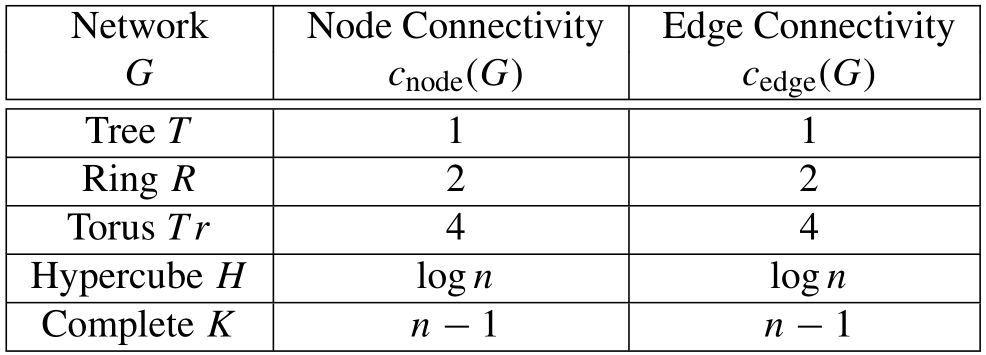
\includegraphics[width=\textwidth]{img/connessioni}
				\end{figure}
			\end{center}
		\end{frame}

\section{Entity failure}

	\logo{}

	\begin{frame}
		\begin{center}
			\Huge{Entity failure}
		\end{center}
		\begin{center}
			\begin{figure}
				
\includegraphics[width=.7\textwidth]{img/panne}
			\end{figure}
		\end{center}
	\end{frame}

	\subsection{Il problema del consenso}
	
		\logo{
\includegraphics[scale=0.02]{img/pasquale}}
	
		\begin{frame}
			\frametitle{p-Consenso}		
			\begin{block}{Problema}
				\begin{itemize}
					\item Ogni entità x ha un valore in input $v(x) \in \mathcal{I}$
					\item Ogni entità deve decidere un valore $d(x) \in \mathcal{O}$ in tempo finito
					\item Una volta scelto $d(x)$ non può più essere modificato
					\item Se tutti i valori $v(x)$ sono uguali, deve essere scelto quel valore
					\item Almeno p entità devono decidere lo stesso valore $d(x)$
					\begin{itemize}
						\footnotesize
						\item $p = N \rightarrow$ \emph{unanimità}
						\item $p = \lceil\frac{N}{2}\rceil +1 \rightarrow$ \emph{maggioranza assoluta}
					\end{itemize}
				\end{itemize}
			\end{block}			
		\end{frame}
	
		\begin{frame}
			\frametitle{Consenso con guasti di tipo crash}	
			Consideriamo solo guasti di tipo crash. Siano $\mathcal{S}$ l'insieme delle entità non guaste, $\mathcal{F}$ l'insieme delle entità guaste e $\mathcal{I} = \mathcal{O} = \{0,1\}$
			\begin{block}{Problema}
				\begin{itemize}
					\item Ogni entità \nguasta ha un valore in input $v(x) \in \mathcal{I}$
					\item Ogni entità \nguasta deve decidere un valore $d(x) \in \mathcal{O}$ in tempo finito
					\item Una volta scelto $d(x)$ non può più essere modificato
					\item Se tutti i valori $v(x)$ iniziali sono uguali, $d(x) = v(x)$ (\emph{non-trivialità})
					\item Vogliamo l'unanimità su tutti gli \nguasta
				\end{itemize}
			\end{block}
		\end{frame}
	
		\begin{frame}
			\frametitle{Consenso con guasti di tipo crash}	
			\begin{block}{Assunzioni}
				\begin{itemize}
					\item La rete è un grafo completo
					\item Link bidirezionali
					\item Sincronia 
					\begin{itemize}
						{\footnotesize
							\item Delay di comunicazione unitari
							\item Clock sincronizzati}
					\end{itemize}
					\item Tutte le entità iniziano la computazione contemporaneamente
					\item L'unico tipo di guasti è CRASH
				\end{itemize}
			\end{block}
		\end{frame}
	
		\begin{frame}
			\frametitle{Protocollo TellZero-Crash}	
			\begin{center}
				\begin{figure}
					\fbox{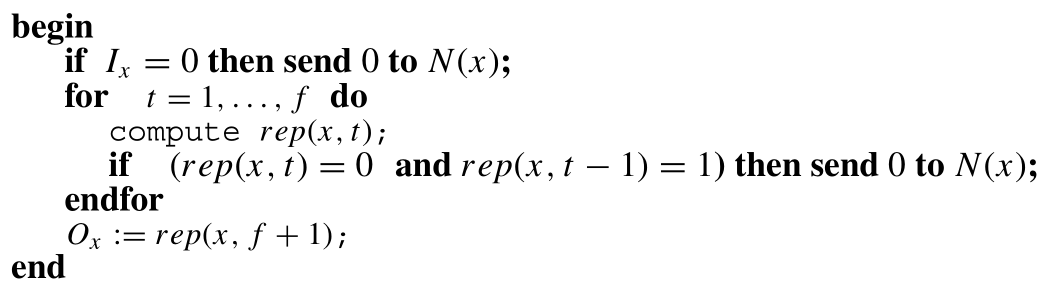
\includegraphics[width=\textwidth]{img/tellZeroCrash}}
				\end{figure}
				\begin{figure}
					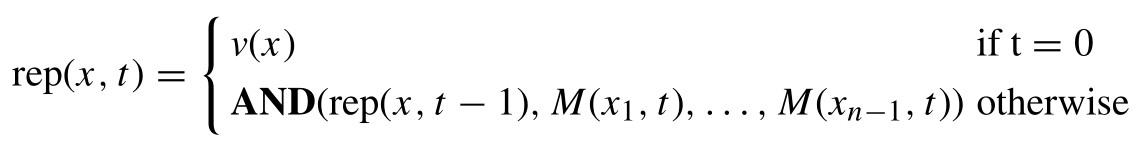
\includegraphics[width=\textwidth]{img/rep}
				\end{figure}
			\end{center}
		\end{frame}
		
		\begin{frame}
			\frametitle{Protocollo TellZero-Crash}	
			\begin{block}{Proprietà}
				\begin{itemize}
					\item Se tutte le entità hanno come valore iniziale 1, tutte le entità \nguasta decideranno 1
					\item Se un'entità \nguasta ha ricevuto o riceve uno 0 al tempo $t < \fint$, allora tutte le entità \nguasta riceveranno uno 0 al tempo $t+1$
					\item Se un'entità \nguasta ha ricevuto o riceve uno 0 durante l'esecuzione del protocollo, allora deciderà 0
				\end{itemize}
			\end{block}
			Riassumendo, ogni entità \nguasta deciderà 0 se almeno una di loro ha come valore iniziale 0 e deciderà 1 se tutte hanno come valore iniziale 1 (\textbf{AND}).
		\end{frame}
	
	\subsection{Consenso in presenza di guasti bizantini}
	
		\begin{frame}
			\frametitle{Guasti bizantini}	
			\begin{block}{Guasto bizantino}
				Un'entità affetta da guasto bizantino può mandare qualunque valore voglia (corretto o errato), in qualunque momento, a qualunque vicino o non mandare niente.				
				Generalmente un guasto bizantino simula un attaccante che cerca di far fallire il protocollo mandando false informazioni o scartando messaggi corretti.
			\end{block}
			\begin{block}{Assunzioni aggiuntive}
				\begin{itemize}
					\item ID unico per ogni entità
					\item Ogni entità conosce l'ID dei suoi vicini
				\end{itemize}
			\end{block}
		\end{frame}
	
		\begin{frame}
			\frametitle{Guasti bizantini}	
			\begin{block}{Consenso}
				Con le precedenti assunzioni si riesce ad arrivare al consenso con un numero di entità bizantine al massimo pari a $(\frac{N}{3}-1)$.
			\end{block}
			Iniziamo a vedere come raggiungere il consenso, inizialmente utilizzando solo valori booleani ($\mathcal{I}=\mathcal{O}=\{0,1\}$)
		\end{frame}
	
		\begin{frame}
			\frametitle{Guasti bizantini}	
			\begin{block}{Formato messaggi}
				\begin{itemize}
					\item \{\textbullet,0,id(s),t\}
					\item s è il mittente del messaggio
					\item id(s) il suo ID univoco
					\item t il passo corrispondente a quando è stato spedito il messaggio
				\end{itemize}
			\end{block} 
			\begin{block}{Problemi con guasti bizantini}
				\begin{enumerate}
					\item \guasta potrebbe mandare \mes{\textbullet}{0}{z}{$t'$} a \nguasta con $t'\neq t$
					\item \guasta potrebbe mandare \mes{\textbullet}{0}{y}{t} a \nguasta con $y \neq z$
					\item \guasta potrebbe mandare informazioni diverse a vicini diversi facendo decidere alcuni 0 e altri 1.
				\end{enumerate}
			\end{block}
		\end{frame}	
		
		\begin{frame}
			\frametitle{RegisteredMail}	
			\begin{block}{Algoritmo}
				Siano $x,y \in \mathcal{S}$, $v(x) = 0$ e sia $z \in \mathcal{F}$
				\begin{itemize}
					\item x manda inizialmente al tempo t \mes{"init"}{0}{x}{t} a tutte le entità
					\begin{itemize}
						\footnotesize
						\item Al tempo $t+1$, y riceve \mes{"init"}{0}{x}{t} e manda \mes{"echo"}{0}{x}{t} a tutte le entità
						\item Al tempo $t' \neq t+1$, y riceve \mes{"init"}{0}{x}{t} ed ignora il messaggio
					\end{itemize}
					\item Al tempo $t' \geq t+2$, y ha ricevuto \mes{"echo"}{0}{x}{t}  da almeno $\fint + 1$ entità diverse e manda \mes{"echo"}{0}{x}{t} (se non lo ha già fatto) al tempo $t'$ a tutte le entità
					\item Al tempo $t' \geq t+1$ y ha ricevuto \mes{"echo"}{0}{x}{t} da almeno $n - \fint$ entità diverse e accetta il messaggio
				\end{itemize}
			\end{block}			
		\end{frame}
	
		\begin{frame}
			\frametitle{RegisteredMail}	
			\begin{block}{Proprietà}
				\begin{enumerate}
					\item se x manda \mes{"init"}{0}{x}{t}, allora il messaggio verrà accettato da tutte le entità non guaste al tempo t+2
					\item se un messaggio è accettato da una qualunque entità non guasta al tempo $t' > t$, allora sarà accettato da tutte le entità non guaste al tempo $t' + 1$
					\item se x non manda \mes{"init"}{0}{x}{t}, allora un eventuale messaggio \mes{"init"}{0}{x}{t} non sarà accettato dalle entità non guaste
				\end{enumerate}
			\end{block}		
		\end{frame}
	
		\begin{frame}
			\frametitle{TellZeroByz}
			\begin{block}{Protocollo}
				\begin{enumerate}
					\item Al tempo 0, ogni entità \nguasta con $v(x) = 0$ avvia RegisteredMail (RM) mandando \mes{"init"}{0}{x}{t}
					\item Al tempo $2i$, $1 \leq i \leq \fint+1$, una entità \nguasta avvia RM mandando \mes{"init"}{0}{x}{$2i$} SSE ha accettato messaggi da almeno $\fint + i - 1$ entità differenti al tempo $2i$ e non ha ancora mandato un messaggio \mes{"init"}{0}{x}{t}
					\item Al tempo $2(\fint + 2)$, una entità \nguasta decide 0 SSE fino a quel momento ha accettato messaggi da almeno $2\fint + 1$ entità diverse. Altrimenti decide 1.
				\end{enumerate}
			\end{block}	
		\end{frame}
	
		\begin{frame}
			\frametitle{TellZeroByz}	
			\begin{block}{Risultato}
				TellZeroByz risolve il problema del consenso con valori booleani in una rete sincrona e completa sotto le restrizioni dichiarate per ogni valore di $\fint \leq \frac{N}{3} - 1$ dopo $2(\fint + 2)$ unità di tempo.
			\end{block}
			Per dimostrare questo risultato dobbiamo dimostrare la non-trivialità e il consenso. 
		\end{frame}
	
		\begin{frame}
			\frametitle{Dimostrazione}	
			\begin{block}{Non-trivialità}
				\begin{itemize}
					\item Se tutte le entità non guaste hanno valore iniziale 0, tutte faranno partire RM al tempo 0 e, per le proprietà del meccanismo, tutte accetteranno i rispettivi messaggi al tempo 2 e decideranno 0 al termine del protocollo.
					\item Se tutte le entità non guaste hanno valore iniziale 1, non faranno mai partire RM. Infatti, per farlo, una entità deve accettare almeno $\fint + 1$ messaggi ma solo le $\fint$ entità guaste possono aver generato tali messaggi. Di conseguenza le entità non guaste decideranno 1 al termine del protocollo.
				\end{itemize}			
			\end{block}
		\end{frame}
	
		\begin{frame}
			\frametitle{Dimostrazione}
			Se un'entità non guasta decide 0, tutte le altre unità non guaste decideranno 0. Supponiamo che \nguasta abbia deciso 0.
			\begin{block}{Consenso caso tutti 0}
				\begin{itemize}
					\item Al tempo $t = 2(\fint + 2)$ x ha accettato messaggi da almeno $2(\fint + 1)$ entità diverse. Sia $\mathcal{R}$ l'insieme delle entità non guaste tra queste.
					\item $|\mathcal{R}| \geq (2\fint + 1) - \fint = \fint + 1$
				\end{itemize}			
			\end{block}
		\end{frame}
	
		\begin{frame}
			\frametitle{Dimostrazione}
			\begin{block}{Consenso caso tutti 0}
				\begin{itemize}
					\item Se tutte le entità in $\mathcal{R}$ hanno valore iniziale 0, ognuna fa partire RM al tempo 0.
					\item Proprietà 1 di RM $\Rightarrow$ tutte le unità non guaste accettano messaggi da $|\mathcal{R}| \geq \fint + 1$ entità al tempo 2.
					\item Proprietà 2 di TZB $\Rightarrow$ ogni entità non guasta farà partire RM.
					\item Proprietà 1 di RM $\Rightarrow$ tutte le unità non guaste accetteranno questi messaggi al tempo 4.
					\item Al tempo $2(\fint + 2) \geq 4$ il protocollo termina e tutte le unità non guaste decidono 0.
				\end{itemize}			
			\end{block}
		\end{frame}
	
		
		\begin{frame}
			\frametitle{Dimostrazione}
			\begin{block}{Consenso caso almeno un 1}
				\begin{itemize}
					\item Se una entità y in $\mathcal{R}$ ha valore iniziale 1, non farà partire RM al tempo 0.
					\item x ha accettato il suo messaggio $\Rightarrow$ y deve aver fatto partire RM a qualche tempo $2i$ con $1 \leq i \leq \fint + 1$
					\item Proprietà 2 di TZB $\Rightarrow$ se y fa partire RM al tempo $2i$ $\Rightarrow$ ha accettato almeno $\fint + i - 1$ messaggi differenti.
					\item Proprietà 2 di RM $\Rightarrow$ gli $\fint + i - 1$ messaggi sono accettati da tutte le unità non guaste al tempo $2i + 1$.
					\item Proprietà 1 di RM $\Rightarrow$ il messaggio originato da y al tempo $2i$ viene accettato da tutte le unità non guaste al tempo $2i+2$.
					\item Ogni unità non guasta accetta almeno $(\fint + i - 1) + 1 = \fint + i$ messaggi al tempo $2i + 2$
				\end{itemize}			
			\end{block}
		\end{frame}
	
		\begin{frame}
			\frametitle{Dimostrazione}
			\begin{block}{Consenso caso almeno un 1}
				\begin{itemize}
					\item $i \leq \fint \Rightarrow$ tutte le unità non guaste che non hanno fatto ancora partire RM, lo faranno al tempo $2i + 2$.  
					\begin{itemize}
						\item Al tempo $2i + 4 \leq 2 \fint + 4 = 2(\fint + 2)$ ogni entità non guasta avrà accettato almeno $n - \fint \geq 2 \fint + 1$ differenti messaggi.
						\item Ogni entità non guasta deciderà 0 al termine del protocollo. 
					\end{itemize}
					\item $i = \fint + 1 \Rightarrow$ tutte le unità non guaste hanno accettato $\fint + i \geq 2\fint + 1$ differenti messaggi al tempo $2(\fint + 1) + 2 = 2(\fint + 2)$  
					\begin{itemize}
						\item Tutte le unità non guaste decideranno 0 al termine del protocollo (adesso).
					\end{itemize}								
				\end{itemize}			
			\end{block}
		\end{frame}
	
		\begin{frame}
			\frametitle{Complessità}
			\begin{block}{Tempo}
				Il protocollo termina sempre in $2(\fint + 2)$ unità di tempo.
			\end{block}
			\begin{block}{Numero di messaggi}
				\begin{itemize}
					\item Ogni \nguasta fa partire RM al più una volta creando $n - 1$ messaggi di "init" e al più $n(n-1)$ messaggi di echo.
					\item Ogni \guasta può mandare messaggi a tutti i vicini ad ogni istante di tempo $\Rightarrow$ $2(\fint + 2)(n-1))$.
					\item Un tempo pari, può essere usato da z per far partire RM generando quindi ulteriori $n(n-1)$ messaggi.
					\item Il numero di messaggi totale è quindi $\mathcal{M}\leq (2\fint^2 + 4\fint + n + n^2 - \fint n + n - \fint)(n-1) = \mathcal{O}(n^3)$
				\end{itemize}			
			\end{block}
		\end{frame}
	
		\begin{frame}
			\frametitle{Oltre TZB}
			\begin{block}{Generalizzazione}
				Esistono algoritmi che generalizzano questi risultati:
				\begin{itemize}
					\item L'algoritmo \emph{FromBoolean(TZB)} generalizza l'insieme di valori in input da Booleano ad arbitrario.
					\begin{itemize}
						\footnotesize
						\item Complessità messaggi $\leq 2n(n-1) + TZB$
						\item Complessità tempo $= 2\fint + 6$
					\end{itemize}
					\item L'algoritmo \emph{ByzComm(TZB)} risolve il problema in una rete sincrona con $C_{node}(G) \geq 2\fint + 1$, $\forall \fint \leq \frac{n}{3} - 1$ ma ogni entità deve conoscere tutta la topologia della rete.
					\begin{itemize}
						\footnotesize
						\item Complessità messaggi $= \mathcal{O}(\fint n^4 \log n)$
						\item Complessità tempo $= \mathcal{O}(\fint n)$
					\end{itemize}
				\end{itemize}
			\end{block}		
		\end{frame}

\section{Link failure}

	\logo{}

	\begin{frame}
		\begin{center}
			\Huge{Link failure}
		\end{center}
		\begin{center}
			\begin{figure}
				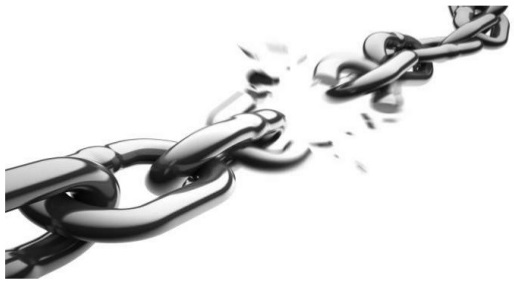
\includegraphics[width=.9\textwidth]{img/link2}
			\end{figure}
		\end{center}
	\end{frame}

	\subsection{Generali sincronizzati}
	
		\logo{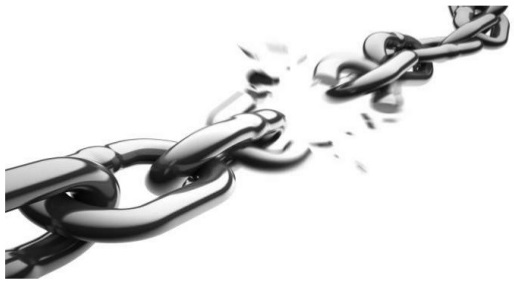
\includegraphics[scale=0.1]{img/link2}}
	
		\begin{frame}
			\frametitle{Il problema dei generali sincronizzati}
			\begin{center}
				\begin{figure}
					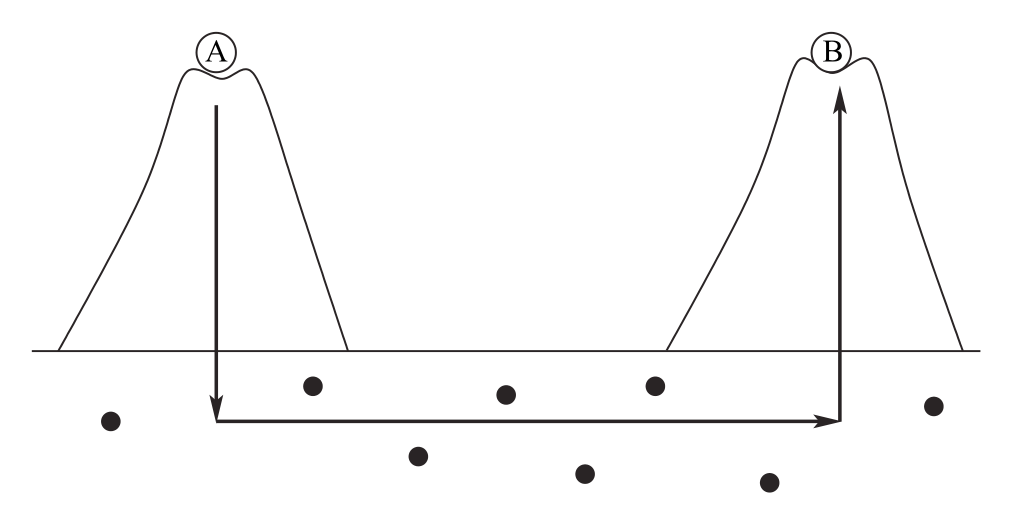
\includegraphics[width=\textwidth]{img/generali}
				\end{figure}			
			\end{center}		
		\end{frame}
	
		\begin{frame}
			\frametitle{I generali sincronizzati}
			\begin{block}{Teorema}
				Il problema dei generali sincronizzati è irrisolvibile. Per raggiungere la \emph{common knowledge}, supponendo che $F$ link possano guastarsi, si ha bisogno che la rete G abbia $C_{edge}(G) \geq F+1$.	
			\end{block}
			In pratica abbiamo bisogno della certezza che ci sia almeno un link tra qualunque coppia di nodi che sicuramente non si guasti.
		\end{frame}
	
	\subsection{Computazione con link guasti}
	
		\begin{frame}
			\frametitle{Broadcasting is the way}
			\begin{block}{Condizioni}
				\begin{enumerate}
					\item Al più $k$ link possono guastarsi
					\item $C_{edge}(G) \geq k+1$
					\item ID univoci (opzionale)
				\end{enumerate}
			\end{block}
			\begin{block}{Soluzione}
				\begin{itemize}
					\item 1 e 2 $\Rightarrow$ broadcast (ad esempio con flood) in sicurezza $\Rightarrow$ possiamo computare funzioni base (AND, OR, Min, Max)
					\item 1,2 e 3 $\Rightarrow$ leader election
				\end{itemize}
			\end{block}		
		\end{frame}
	
	\subsection{Broadcast in una rete completa con link guasti}
		
		\begin{frame}
			\frametitle{Numero di guasti}
			\begin{block}{Costo}
				Broadcast in un grafo completo senza guasti è banale e costa $(n-1)$ messaggi. Consideriamo di avere sugli $\frac{n(n-1)}{2}$ collegamenti, $\fint < n-1$ guasti
				\begin{itemize}
					\item Non conosciamo $\fint$
					\begin{itemize}
						\item Con Flood risolviamo il problema ma ci costa $(n-1)^2$ messaggi
					\end{itemize}
					\item Conosciamo $\fint$ a priori
					\begin{itemize}
						\item Con \emph{TwoSteps} possiamo abbassare questo costo.
					\end{itemize}
				\end{itemize}				
			\end{block}
		\end{frame}
	
		\begin{frame}
			\frametitle{TwoSteps}
			\begin{block}{Algoritmo}
				\begin{enumerate}
					\item x vuole far arrivare a tutti il valore $v$ e manda un messaggio \{ Info, v \} a $\fint + 1$ vicini
					\item Una entità y che riceve un messaggio \{ Info, v \} da x, manda \{ Echo, v \} a tutti i suoi vicini
				\end{enumerate}				
			\end{block}
		\end{frame}
	
		\begin{frame}
			\frametitle{TwoSteps}
			\begin{block}{Correttezza}
				\begin{itemize}
					\item $y \neq x$ non riceve il messaggio Info da x a causa del link (x, y) guasto
					\item Sia $p(x) \leq k$ il numero di link guasti incidenti x.
					\item Al primo passo, almeno $n - 1 - p(x)$ vicini riceveranno il messaggio Info di x
				\end{itemize}				
			\end{block}
			\begin{center}
				\begin{figure}
					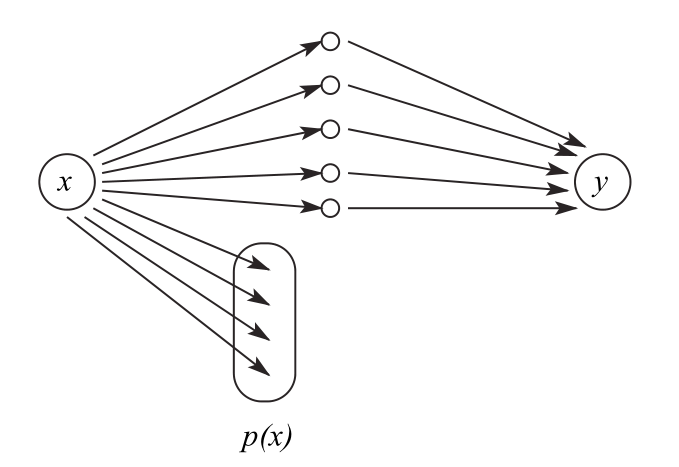
\includegraphics[scale=0.35]{img/twoSteps}
				\end{figure}
			\end{center}
		\end{frame}
	
		\begin{frame}
			\frametitle{TwoSteps}
			\begin{block}{Correttezza}
				\begin{itemize}
					\item Al secondo passo, tutti loro manderanno il messaggio Echo a tutti i loro vicini, incluso y
					\item Almeno $n - 1 - p(x)$ messaggi di Echo verranno mandati a y e al più $\fint - p(x)$ link saranno guasti
					\item $n-1 > \fint \Rightarrow n - 1 - p(x) > \fint - p(x) \Rightarrow$ almeno un Echo arriva ad y  
				\end{itemize}				
			\end{block}
			\begin{center}
				\begin{figure}
					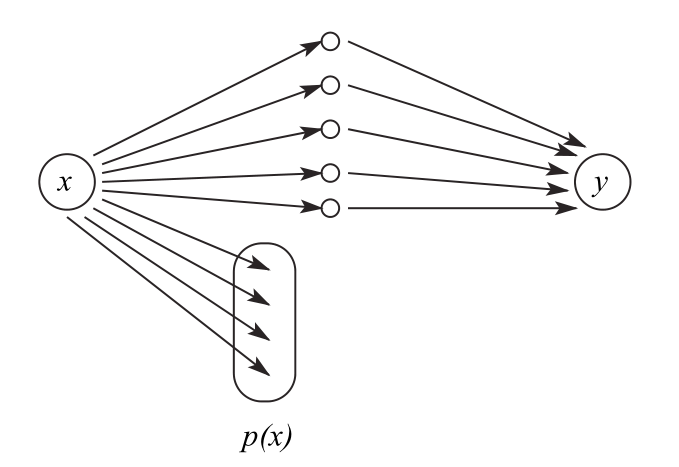
\includegraphics[scale=0.32]{img/twoSteps}
				\end{figure}
			\end{center}
		\end{frame}
	
		\begin{frame}
			\frametitle{TwoSteps}
			\begin{block}{Costo}
				\begin{itemize}
					\item Al primo passo x manda $\fint+1$ messaggi
					\item Al secondo passo, al più $\fint+1$ entità mandano ognuna $n-2$ messaggi
					\item $(\fint+1)+(\fint+1)(n-2) = (\fint+1)(1 + n - 2) = (\fint+1)(n-1)$
				\end{itemize}			
			\end{block}
			Dato che $\fint \leq n-2$ il numero di messaggi scambiato da TwoSteps è minore di Flood.
		\end{frame}
	
		\begin{frame}
			\frametitle{Leader election}
			Supponiamo sempre $\fint < n - 1$ e che ogni entità abbia un ID unico.
			\begin{block}{FT-BcastElect}
				\begin{enumerate}
					\item Ogni entità x manda in broadcast con un protocollo fault tolerant (ad esempio con TwoSteps) il suo valore id(x)
					\item Una volta che x ha ricevuto tutti i valori di tutte le altre entità, x diventa leader SSE il suo id è il minimo
				\end{enumerate}			
			\end{block}
			\begin{block}{Costo}
				Tutti gli n nodi eseguono TwoSteps quindi il numero di messaggi scambiato è $\leq n(\fint+1)(n-1)$
			\end{block}
		\end{frame}
	
		\begin{frame}
			\frametitle{Conclusioni}
			\begin{block}{Difficile ma non impossibile}
				\begin{itemize}
					\item I guasti accadono, dobbiamo conviverci
					\item Gli algoritmi funzionanti in presenza di guasti sono corretti ma spesso costosi (sia in termine di messaggi che di infrastrutture necessarie)
					\item Esistono casi particolari nei quali, sotto opportune condizioni, si riescono a raggiungere buoni risultati con costi contenuti
				\end{itemize}	
			\end{block}
		\end{frame}